Chaque sommet de $G_{k,k'}$ est identifi\'e par le couple $(i,j)$ avec $0 \le i < k$ et $0 \le j < k'$. Le sommet $(i,j)$ est adjacent  au sommet :
\begin{itemize}
	\item $(i, j+1)$ si $j < k'-2$
	\item $(i+1,j)$ si $i < k-2$
	\item $(i,j-1)$ si $j > 0$
	\item $(i-1,j)$ si $i > 0$
\end{itemize}
De plus, les sommets  $(0,0)$ et $(0,k-1)$,  $(0,0)$ et $(0,k'-1)$ , $(k-1,0)$ et $(k-1,k'-1)$, $(0,k'-1)$ et $(k-1,k'-1)$ sont adjacents.
On remarque que tout graphe  induit par un sommet et son voisinage forme un graphe \'etoile $K_{1,4}$.
La figure \ref{exempleGrapheCellule} est un exemple de {\em grille boucl\'ee} $G_{4,4}$. Ce graphe contient $16$ sommets, $28$ ar\^etes. Les sommets $(0,0), (0,1), (1,1), (1,0)$ forme une cellule et le graphe $G_{4,4}$ contient  $10$ cellules. 
% ---- figure exemple graphe cellule G_{4,4}
\begin{figure}[htb!] 
\centering
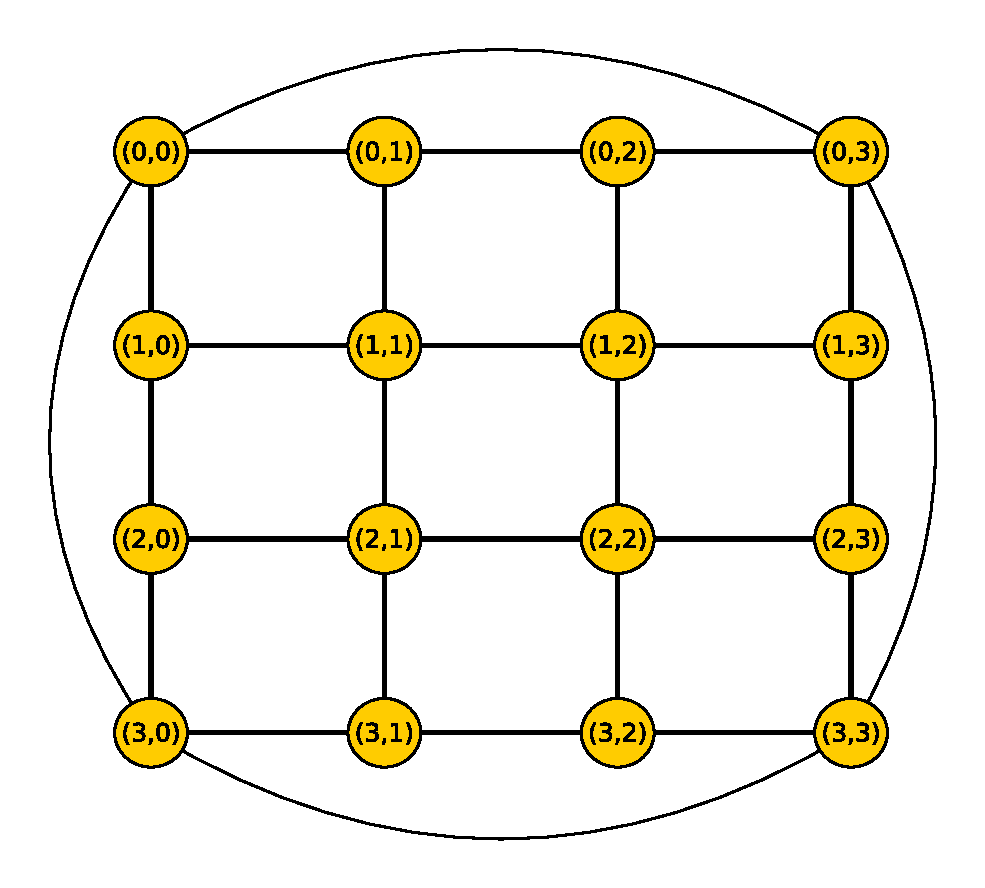
\includegraphics[scale=0.6]{exempleGrapheCelluleG33.eps}
\caption{ La grille boucl\'ee $G_{4,4}$ : elle est compos\'ee de $16$ sommets, $28$ ar\^etes et $10$ cellules. }
\label{exempleGrapheCellule} 
\end{figure}
%\FloatBarrier
% ---- figure exemple graphe cellule G_{4,4}
\begin{definition}
Une cellule est un cycle de longueur $4$ identifi\'e par les sommets $(i,j)$, $(i,j+1)$, $(i+1,j)$ et $(i+1,j+1)$ avec $i<k-1$ et$j<k'-1$. Nous notons une telle cellule $C_{i,j}$.
\end{definition}
Si $k = k' = 2$, la grille boucl\'ee $G_{2,2}$ est la cellule $C_{0,0}$.

\begin{property}
Le graphe $G_{k,k'}$ poss\`ede $k \times k'$ sommets,  $k \times (k'-1) + k' \times(k-1) + 4$  ar\^etes et $(k-1) \times (k'-1) +1$ cellules.
\end{property}




%Deux sommets de lignes diff\'erentes partagent une ar\^ete si les lignes sont consecutives de la maniere suivante: 
%Deux sommets partagent une ar\^ete si :
%\begin{itemize}
%\item les sommets appartiennent \`a la m\^eme ligne et \`a des colonnes successives. 
%\item les sommets sont de lignes successives mais de la m\^eme colonne.
%\end{itemize}
%Par exemple, soit le sommet $(i,j)$ \`a la ligne $i$ et la colonne $j$. Le sommet $(i+1,j)$ appartient \`a la ligne $i+1$ et la colonne $j$. De m\^eme, les sommets $(i,j+1)$ et $(i+1,j+1)$ appartiennent \`a la colonne $j+1$ mais ils sont respectivement de la ligne $i$ et de la ligne $i+1$. Il existe une ar\^ete entre les sommets $(i,j)$ et $(i+1,j)$. 
%Nous notons $\{(i,j)$,$(i+1,j)\}$ cette ar\^ete avec $i<k-1$ et $j< k'-1$. 
%De m\^eme, les ar\^etes entre les sommets  $(i,j+1)$ et $(i+1,j+1)$, $(i,j)$ et $(i+1,j)$, $(i+1,j)$ et $(i+1,j+1)$ sont not\'ees, respectivement $\{(i,j+1), (i+1,j+1)\}$, $\{(i,j),(i+1,j)\}$, $\{(i+1,j),(i+1,j+1)\}$.
%Nous rappelons que  $i<k-1$ et $j< k'-1$.
%Ainsi, $i=k-1$ et $j = k'-1$, nous ajoutons les ar\^etes suivantes $\{(0,0),(0,k-1)\}$, $\{(0,0),(0,k'-1)\}$, $\{(k-1,0),(k-1,k'-1)\}$, $\{(0,k'-1),(k-1,k'-1)\}$.
%\newline
%Dans ce graphe, aucun voisin d'un sommet n'est couvert par $2$ cliques. En effet, le graphe induit par ce sommet et son voisinage forme un graphe {\em \'etoile} $K_{1,4}$.
%
%\begin{definition}
%Une cellule est un cycle de longueur $4$ identifi\'e par les sommets $(i,j)$, $(i,j+1)$, $(i+1,j)$ et $(i+1,j+1)$ avec $i<k-1$ et$j<k'-1$. Nous notons la cellule $C_{i,j}$.
%\end{definition}
%Si $k = k' = 2$, la grille boucl\'ee $G_{2,2}$ est la cellule $C_{0,0}$.
%
%\begin{property}
%Le graphe $G_{k,k'}$ poss\`ede $k \times k'$ sommets,  $k \times (k'-1) + k' \times(k-1) + 4$  ar\^etes et $(k-1) \times (k'-1) +1$ cellules.
%\end{property}
%
%
%
%Dans la figure \ref{exempleGrapheCellule}, nous avons un exemple de la grille boucl\'ee $G_{4,4}$ avec $k=4$ et $k'=4$. Nous avons $16$ sommets, $28$ ar\^etes et $10$ cellules. 
%
%
%%Soient $n$ et $m$ deux entiers tels que $n < k$ et $m < k'$.
%%Consid\'erons une cellule $G_{n,m}$ qui contient $4$ sommets et $4$ ar\^etes.
%%Les sommets de  $G_{n,m}$  sont not\'es par les couples $(n,m)$, $(n,m+1)$, $(n+1,m)$,  $(n+1,m+1)$. 
%%
%%% -----
%%Nous d\'esignons par 
%%\begin{itemize}
%%\item $e_{n} = \{(n,m),(n,m+1)\}$ l'ar\^ete entre les sommets $(n,m)$ et $(n,m+1)$,   
%%\item $e_{m} = \{(n,m),(n+1,m)\}$ l'ar\^ete entre les sommets $(n,m)$ et $(n+1,m)$,   
%%\item $e_{n+1} = \{(n+1,m),(n+1,m+1)\}$ l'ar\^ete entre les sommets $(n+1,m)$ et $(n+1,m+1)$,   
%%\item $e_{m+1} = \{(n,m+1),(n+1,m+1)\}$ l'ar\^ete entre les sommets $(n,m+1)$ et $(n+1,m+1)$.
%%\end{itemize}
%%Nous faisons varier $n$ et $m$ par pas de $1$ et nous s\'electionnons les cellules $G_{n,m}$ et $G_{n,m+1}$.
%%L'ar\^ete $e_{m+1}$ est commune aux cellules $G_{n,m}$ et $G_{n,m+1}$. 
%%De m\^eme, les cellules $G_{n,m}$ et $G_{n+1,m}$ partagent l'ar\^ete $e_{n+1}$. 
%%Ainsi, \`a chaque \'etape de la construction, chaque cellule partage 
%%$2$ ar\^etes si $n = m = 0$ ou $n = k-1 ~et~ m = k'-1$,
%%$3$ ar\^etes si $n = \{0,k-1\} ~et~ m \neq \{0,k'-1\}$ ou $m = \{0,k'-1\} ~et~ n \neq \{0,k-1\}$, 
%%$4$ ar\^etes si $n \neq \{0,k-1\} ~et~ m \neq \{0,k'-1\}$. 
%%\newline
%%\`A la fin de la boucle, nous ajoutons les ar\^etes $\{(0,0),(k+1,0)\}$, $\{(0,0),(0,k+1)\}$, $\{(k+1,k'+1),(k+1,0)\}$ et $\{(k+1,k'+1),(0,k+1)\}$.
%%Nous obtenons ainsi le graphe $G_{k,k'}$.
%%% -----
%%
%%\begin{definition}
%%Le graphe $G_{k,k'}$ poss\`ede $(k+1) \times (k'+1)$ sommets,  $k \times (k'+1) + k' \times(k+1) + 4$  ar\^etes et $k \times k' +1$ cellules.
%%\end{definition}
%%
%%% ---- figure exemple graphe cellule G_{3,3}
%%\begin{figure}[htb!] 
%%\centering
%%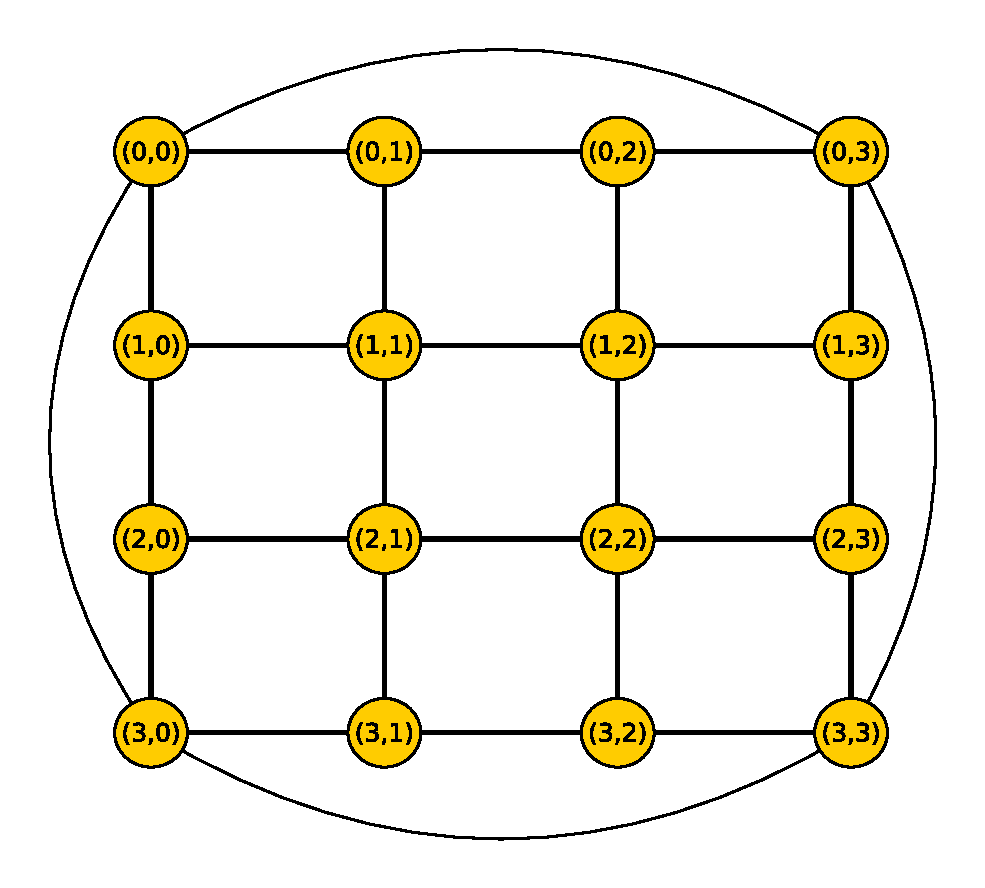
\includegraphics[scale=0.6]{exempleGrapheCelluleG33.eps}
%%\caption{ Le graphe cellule $G_{3,3}$ : il est compos\'e de $16$ sommets, $28$ ar\^etes et $9$ cellules. }
%%\label{exempleGrapheCellule} 
%%\end{figure}
%%%\FloatBarrier
%%% ---- figure exemple graphe cellule G_{3,3}
%%
%%Dans la figure \ref{exempleGrapheCellule}, nous avons un exemple de graphe cellule $G_{3,3}$ avec $k=3$ et $k'=3$. Nous avons $16$ sommets, $28$ ar\^etes et $9$ cellules. 